\documentclass[letterpaper]{article}

\usepackage[margin=1.5in]{geometry}

\usepackage{styles/packages}



% Author info
\title{Title Here}
\author{%
	Author One$^1$%\thanks{}%
	\and%
	Author Two$^1$% 
	\and% 
	Author Three$^1$%
}

\date{
	$^1$Saint Martin's University \\ %
	\texttt{%
		% auth1@stmartin.edu, \\%
		% auth2@stmartin.edu, \\%
		% auth3@stmartin.edu%
	}\\[2ex]%
	% $^2$Organization 2 \\ \texttt{email}\\[2ex]%
	\today
}

\addbibresource{bibliography.bib}

\begin{document}
\maketitle

\begin{abstract}
	\lipsum[1]

	% \noindent\textbf{Keywords:} keywords, separated, by, commas
\end{abstract}

\tableofcontents

\section{Introduction and Background}
\label{sec:intro}

Introduce the project and give some background, including a description of a literature search for related projects. Here's how to cite \autocite[p.~23]{Russell2020}. 

\subsection{Here's a subsection}
\label{sec:subsection-label}

\lipsum[5]

\subsection{Here's another subsection}

Kind of like \cref{sec:subsection-label}.

\lipsum[5]

\section{Design}
\label{sec:design}

If there is a design component to the project, include this section and describe the design. The idea isn't to tell a history of what you did but to describe the result of the design itself.

\lipsum[4]

\section{Methods}
\label{sec:methods}

This is where the methods used to conduct the project can be described. If it is a design project, this is where you analyze the design (but save the results of the analysis for the next section).

This section can also include a description of materials used.

An equation should be part of a sentence, like
\begin{equation} \label{eq:x}
\bm{x} = \begin{bmatrix}
3 & -5 \\
4 & 0
\end{bmatrix}
\bm{y} +
\bm{b}.
\end{equation}
Refer to equations like \cref{eq:x} like this.

\lipsum[6]

\section{Results}
\label{sec:results}

Present the results of \cref{sec:methods}, including figures and important data. Stick to the facts without interpretation. Insert figures like \cref{fig:expert} as shown in this source, below.

\begin{figure}[htbp]
\centering
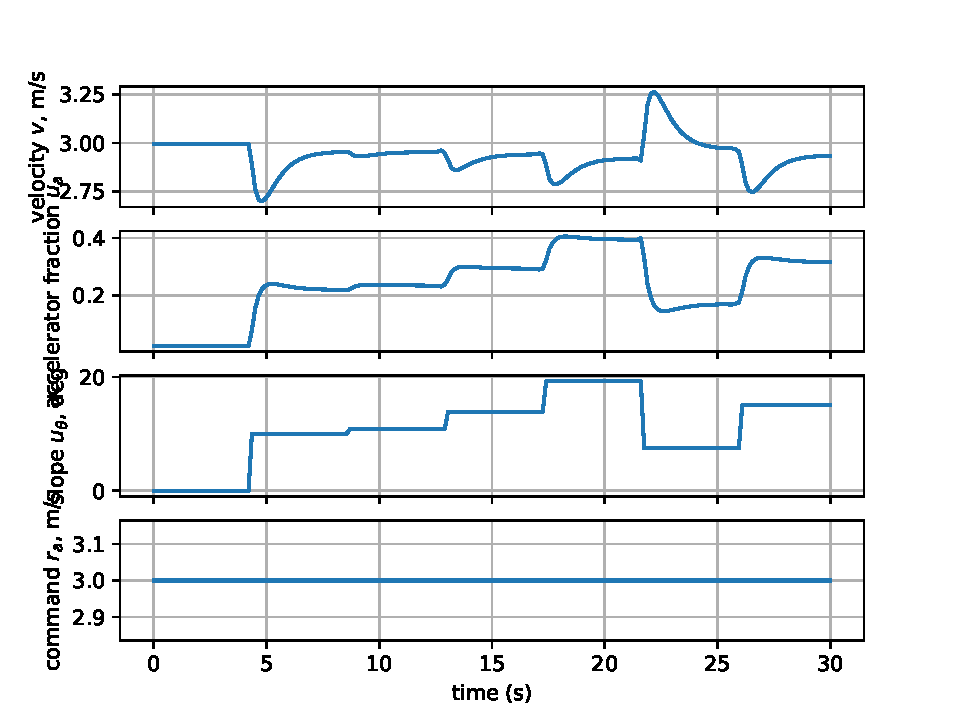
\includegraphics[width=1\linewidth]{figures/expert-0035.pdf}
\caption{Write a caption describing the figure.}
\label{fig:expert}
\end{figure}

\lipsum[5]

\section{Discussion}
\label{sec:discussion}

Discuss and interpret the results from \cref{sec:results}.

\lipsum[3]

\section{Conclusion}
\label{sec:conclusion}

Conclude. Explain what we learned.

\lipsum[2]

% \paragraph{Acknowledgements} \lipsum[6]

\section*{Bibliography}
\addcontentsline{toc}{section}{Bibliography}
\printbibliography[heading=none]

\appendix

\section{Additional Topic}
\label{app:1}

This is optional, but perhaps something is interesting but would break up the flow of the report. Include more than one appendix, if needed.

\lipsum[8]
	
\end{document}